\documentclass{article}
\setlength{\parskip}{5pt} % esp. entre parrafos
\setlength{\parindent}{0pt} % esp. al inicio de un parrafo
\usepackage{amsmath} % mates
\usepackage[sort&compress,numbers]{natbib} % referencias
\usepackage{url} % que las URLs se vean lindos
\usepackage[top=25mm,left=20mm,right=20mm,bottom=25mm]{geometry} % margenes
\usepackage{hyperref} % ligas de URLs
\usepackage{graphicx} % poner figuras
\usepackage[spanish]{babel} % otros idiomas
\usepackage[utf8]{inputenc}
\usepackage{wrapfig}
\usepackage{listings}
\usepackage{xcolor}
\usepackage{subfig} 
\definecolor{codegreen}{rgb}{0,0.6,0}
\definecolor{codegray}{rgb}{0.5,0.5,0.5}
\definecolor{codepurple}{rgb}{0.58,0,0.82}
\definecolor{backcolour}{rgb}{0.95,0.95,0.92}
 
\lstdefinestyle{mystyle}{
    backgroundcolor=\color{backcolour},   
    commentstyle=\color{codegreen},
    keywordstyle=\color{magenta},
    numberstyle=\tiny\color{codegray},
    stringstyle=\color{codepurple},
    basicstyle=\footnotesize,
    breakatwhitespace=false,         
    breaklines=true,                 
    captionpos=b,                    
    keepspaces=true,                 
    numbers=left,                    
    numbersep=5pt,                  
    showspaces=false,                
    showstringspaces=false,
    showtabs=false,                  
    tabsize=2
}
\lstset{style=mystyle}
\lstset{language=Python}
\author{Equipo 4 \\Jorge  Fuentes, Tania  Hernandez,
 Anahi Herrera, Gustavo  Díaz, Miriam  Mata, Alejandro Ramos} % author
\title{Práctica 5 \\ Optimización de una prótesis de pie} % titulo
\date{\today}

\begin{document} % inicia contenido
\maketitle % cabecera
\begin{abstract} % resumen
\textbf{Objetivo:} El estudiante deberá presentar una propuesta de análisis de formas y de la programación para la ejecución de la optimización (descripción funcional) de características de trabajo especificas que presenta la(s) ventaja(s) (mencionar ventajas). La tecnología en las prótesis ha sido objeto de una transformación sustancial en las últimas décadas, sobre todo con la introducción de materiales y mecanismos elásticos pero también en la geometría, la masa, la alineación. Con el pasar de los años y el avance tecnológico la mayor parte de las prótesis contienen rasgos más humanos, obteniendo múltiples ventajas para proporcionar una segunda oportunidad a personas que han perdido una de sus extremidades. Por esta razón el  documento trata sobre el estudio de los diferentes avances obtenidos hasta la actualidad, los cuales brindan un mejor estilo de vida a la persona.
\end{abstract}
\newpage
\tableofcontents
\newpage
\section{Introducción}\label{intro} % seccion y etiqueta
Las prótesis de pie se tratan de aparatos médicos destinados a sustituir de forma artificial un pie, tobillo o parte del pie faltante en el cuerpo de un paciente a causa de una amputación total o parcial del miembro.\\
Un pie protésico se trata de un aparato médico diseñado justo a la medida de cada paciente para suplantar estética y funcionalmente la parte faltante de la extremidad a causa de una amputación.\\
Esta tiene la función tanto de aparentar que existe la sección faltante como de ser un punto de apoyo para que el paciente pueda caminar, utilizar calzado y desempeñar sus labores de forma normal o lo más normal posible.\\
Las prótesis de pie tienen costos personalizados que dependen de las necesidades de cada paciente, el nivel de amputación y de los materiales y componentes mecánicos que tengan como aditamentos para el movimiento.
%\cite{ff2} CITAR FUENTE

%\begin{figure} % figura
    %\centering
    %\includegraphics[width=150mm]{output3.jpg} % archivo
    %\caption{resultados del programa}
    %\label{grafica}
%\end{figure}
\section{Desarrollo}
\subsection{Nombre y definición de la forma geometría}
\subsubsection{Prótesis de pie}
Es común al momento sufrir una amputación, el  reemplazar el miembro por una extremidad artificial; una protesis. La selección de una prótesis es altamente dependiente de las necesidades y capacidades de cada el paciente. Su función puede variar de puramente estética a una necesidad funcional para un paciente que desea recuperar la independencia en realizar actividades de la vida diaria, o ya sea en el campo deportivo.\\
La tecnología en las prótesis ha sido objeto de una transformación sustancial en las últimas décadas, sobre todo con la introducción de materiales y mecanismos elásticos pero también en la geometría, la masa, la alineación. Con el pasar de los años y el avance tecnológico la mayor parte de las prótesis contienen rasgos más humanos, obteniendo múltiples ventajas para proporcionar una segunda oportunidad a personas que han perdido una de sus extremidades\cite{rf1}. Por esta razón el  documento trata sobre el estudio de los diferentes avances obtenidos hasta la actualidad, los cuales brindan un mejor estilo de vida a la persona.
\subsubsection{Prótesis Biónica} Este tipo de pies protésicos deben contener múltiples adaptaciones y  propiedades de rigidez al caminar, Además, de proporcionan un alto torque a la salida. Durante la fase de impulsión, la posición de la articulación del tobillo debe ser controlado con el fin de evitar la caída del pie en contacto con el talón. Esta es un prototipo de una TT (PPAMs)”Prótesis de pie con músculos artificiales”. El prototipo TT está equipada con tres PPAMs; uno se coloca en frente, dos se colocan en la parte posterior y su trabajo es de forma paralela. Una gama de tobillo se establece de movimiento de 30 grados. La  prótesis consiste tanto en una rodilla articulada y la articulación del tobillo. Dos cilindros neumáticos se utilizan para tener la extremidad inferior de la prótesis completa. Este es un prototipo de una TT (PPAMs).
\newpage
\subsubsection{Prótesis Sach}El pie SACH no soporta mucha carga en la zona de los dedos. Esta falta de apoyo del dedo del pie crea una experiencia de "drop-off". El pie SACH está hecho de una quilla de madera cubierto por espuma de poliuretano\cite{rf2}. Este pie se caracteriza por  ser rígido en el región de madera (media del pie), y por ser bastante flexible en la espuman (zona de los dedos). Estas características se reflejan en el roll-over forma obtenida por el PFLA Una concha de pie polietileno reforzado se usa como un cosmético cubierto. Esta estructura produce una constante, sobre la forma del talón al dedo del pie, lo que se traduce en una constante, el apoyo continuo de peso. Los PFLA está diseñado de modo que una fuerza aplicada al final de la viga se duplica más o menos en el punto de contacto con el pie protésico. Este punto de contacto es proporcionado por un diseño personalizado de la placa  aluminio.\\
Son algunas de las tipos de prótesis investigadas, respecto a los tipos de forma que pueden existir dependiendo de las necesidades del paciente.
\begin{figure}[htp] % figura
    \centering
    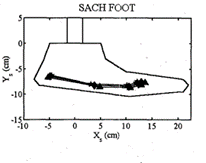
\includegraphics[width=150mm]{piecito.png} % archivo
    \caption{Prótesis Sach.}
    \label{grafica}
\end{figure}
\newpage
\subsection{Estado del arte}
Las prótesis de pie se tratan de aparatos médicos destinados a sustituir de forma artificial un pie, tobillo o parte del pie faltante en el cuerpo de un paciente a causa de una amputación total o parcial del miembro.
Estos aparatos protéticos tienen tanto finalidades funcionales para la rehabilitación del paciente como funciones estéticas sumamente avanzadas para imitar de forma bastante realista la parte del cuerpo faltante.
Los pies son una de las extremidades más importantes y básicas no sólo para poder caminar, sino para simplemente poder sostenerse parado y tener el equilibrio necesario para todo tipo de actividades, por lo que las prótesis de pie y tobillo son de las más importantes y avanzadas en casos de amputación por accidentes, enfermedades o agenesia\cite{rf3}.
Actualmente existe una enorme variedad de prótesis según las necesidades y características de cada persona, así como el tipo de amputación y muñon, por lo que es importante que las conozcas para determinar cuál es la mejor para ti como paciente o para alguna persona conocida que la necesite.\\
Dependiendo del tipo de amputación, la prótesis podrá estar compuesta de diversos elementos, como lo pueden ser:
\begin{itemize}
    \item Socket o encaje con el muñón.
    \item Plantillas.
    \item Almohadillas.
    \item Estabilizadores para el talón.
    \item Elementos estéticos.
\end{itemize}
De igual manera, existen prótesis mucho más avanzadas que pueden tener dispositivos y elementos robóticos, mecánicos, mioeléctricos y biomecánicos para otorgar movimientos especiales en caso de ser necesario.
\subsubsection{Materiales de las prótesis de pie}
El pie prostético puede ser fabricado de uno o más materiales, los cuales son seleccionados para brindar el soporte, agarre y diseño necesario para suplantar la parte faltante del cuerpo humano.
Por lo general de utiliza:
\begin{itemize}
    \item Silicona médica.
    \item Plantillas de carbono.
    \item Rellenos de materiales elásticos.
    \item Aluminio.
    \item Titanio.
    \item Acero inoxidable.
    \item Plásticos.
\end{itemize}
\newpage
\subsection{Propuesta de la geometría, alcances y limitaciones.}
Después de un análisis de esfuerzos, costos de fabricación, facilidad de construcción, ventajas y desventajas que presentaban los prediseños realizados de la prótesis de pie se llegó a un diseño final que tiene como ventaja un análisis de ingeniería en cuanto a sus características físicas y mecánicas para darle un mayor confort al usuario y poder garantizar su perfecto funcionamiento.\\
Para el diseño de cada una de las piezas que conforman la prótesis del pie se tuvo en cuenta algunos diseños realizados por compañías dedicadas exclusivamente a la fabricación de prótesis con el fin de hacer que la prótesis fuera modular y así poder adaptarse fácilmente a las prótesis existentes en el mercado.\\
Para poder realizar nuestra simulación se basó en la información siguiente: 
Se realizó un primer boceto y basados en éste se empezaron a realizar modificaciones, para que fuera más ergonómica y funcional. A partir del diseño básico (siguiente figura) se empezaron a analizar las dimensiones pertinentes teniendo en cuenta los parámetros de antropometría del pie, según las dimensiones del grupo objetivo y  la forma de los huesos del  pie  de acuerdo con el esqueleto humano.
\begin{figure}[htp] % figura
    \centering
    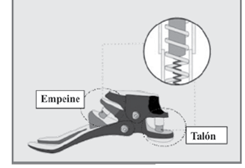
\includegraphics[width=150mm]{boceto 1.png} % archivo
    \caption{Primer boceto del pie.}
    \label{grafica}
\end{figure} 
\newpage
A partir de este boceto se empezaron a realizar cambios sustanciales en el diseño, para poder suplir las necesidades y, de igual manera, cumplir con los objetivos planteados. Para el segundo boceto se redujo la abertura de la planta y se quitó el doble sistema de amortiguación dejando solamente el resorte de nitinol con una sola articulación a nivel del tobillo (siguiente figura).
\begin{figure}[htp] % figura
    \centering
    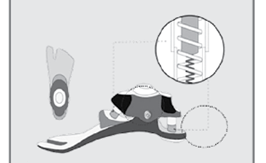
\includegraphics[width=150mm]{boceto 2.png} % archivo
    \caption{Segundo boceto del pie.}
    \label{grafica}
\end{figure}
\subsubsection{Alcances y limitaciones} 
Alcances:
\begin{itemize}
    \item Diseño, simulación y análisis de la prótesis de pie sin llegar a la construcción de un prototipo físico.
    \item En el proceso de selección de materiales, se buscará un diseño con materiales económicos que permitan cumplir con las exigencias del diseño.
    \end{itemize}
Limitaciones:  
\begin{itemize}
    \item Todos los cálculos se realizarán tomando como base la marcha en un plano horizontal.
    \item Se desarrollará un diseño para adultos tomando como referencia los estándares físicos masculinos de la población colombiana.
    \item 	Para el análisis, se tendrán en cuenta que la prótesis de pie solo tiene un grado de libertad. 
\end{itemize}
\newpage
\subsection{Pasos del desarrollo de la programación}
A continuación, veremos la codificación de la programación en MATLAB.
\begin{lstlisting}
%%%% A 99 LINE TOPOLOGY OPTIMIZATION CODE BY OLESIGMUND, OCTOBER 1999 %%%
function topp5a(nelx,nely,volfrac,penal,rmin);
% INITIALIZE
x(1:nely,1:nelx) = volfrac;
loop = 0;
change = 1.;
% START ITERATION
while change > 0.01
   loop = loop + 1;
   xold = x;
   % FE-ANALYSIS
    [U]=FE(nelx,nely,x,penal);
    % OBJECTIVE FUNCTION AND SENSITIVITY ANALYSIS
     [KE] = lk;
      c = 0.;
      for ely = 1:nely
         for elx = 1:nelx
          n1 = (nely+1)*(elx-1)+ely;
          n2 = (nely+1)* elx +ely;
          dc(ely,elx)=0.;
          for i=1:5
              Ue = U([2*n1-1;2*n1; 2*n2-1;2*n2; 2*n2+1; 2*n2+2;
                  2*n1+1;2*n1+2],i);
              c = c + x(ely,elx)^penal*Ue'*KE*Ue;
              dc(ely,elx) = dc(ely,elx)-penal*x(ely,elx)^(penal-1)*Ue'*KE*Ue;
          end
         end
      end
     % FILTERING OF SENSITIVITIES
     [dc] = check(nelx,nely,rmin,x,dc);
     % DESIGN UPDATE BY THE OPTIMALITY CRITERIA METHOD
     [x] = OC(nelx,nely,x,volfrac,dc);
     % PRINT RESULTS
     change = max(max(abs(x-xold)));
     disp(['It.:' sprintf('%4i',loop) 'Obj.:' sprintf('%10.4f',c) ...
         ' Vol.: ' sprintf('%6.3f',sum(sum(x))/(nelx*nely)) ...
         ' ch.: ' sprintf('%6.3f',change )])
     % PLOT DENSITIES
     colormap(gray); imagesc(-x); axis equal; axis tight;
end
%%%%%%%%%% OPTIMALITY CRITERIA UPDATE %%%%%%%%%
function [xnew]=OC(nelx,nely,x,volfrac,dc)
l1 = 0; l2 = 100000; move = 0.2;
while (l2-l1 > 1e-4)
    lmid = 0.5*(l2+l1);
    xnew = max(0.001,max(x-move,min(1.,min(x+move,x.*sqrt(-dc./lmid)))));
    if sum(sum(xnew)) - volfrac*nelx*nely > 0;
        l1 = lmid;
    else
        l2 = lmid;
    end
end
%%%%%%%%%% MESH-INDEPENDENCY FILTER %%%%%%%%%%%
function [dcn]=check(nelx,nely,rmin,x,dc)
dcn=zeros(nely,nelx);
for i = 1:nelx
    for j = 1:nely
        sum=0.0;
        for k = max(i-round(rmin),1):min(i+round(rmin),nelx)
            for l = max(j-round(rmin),1):min(j+round(rmin), nely)
                fac = rmin-sqrt((i-k)^2+(j-l)^2);
                sum = sum+max(0,fac);
                dcn(j,i) = dcn(j,i) + max(0,fac)*x(l,k)*dc(l,k);
            end
        end
        dcn(j,i) = dcn(j,i)/(x(j,i)*sum);
    end
end
%%%%%%%%%% FE-ANALYSIS %%%%%%%%%%%%
function [U]=FE(nelx,nely,x,penal)
[KE] = lk;
K = sparse(2*(nelx+1)*(nely+1), 2*(nelx+1)*(nely+1));
F = sparse(2*(nely+1)*(nelx+1),5); U =sparse(2*(nely+1)*(nelx+1),5);
for ely = 1:nely
    for elx = 1:nelx
        n1 = (nely+1)*(elx-1)+ely;
        n2 = (nely+1)* elx +ely;
        edof = [2*n1-1; 2*n1; 2*n2-1; 2*n2; 2*n2+1;2*n2+2;2*n1+1; 2*n1+2];
        K(edof,edof) = K(edof,edof) + x(ely,elx)^penal*KE;
    end
end
% DEFINE LOADSAND SUPPORTS(HALF MBB-BEAM)
F(3222,1) = -1;
F(3782,2) = -1;
F(2662,3) = -1;
F(2942,4) = -1;
F(3502,5) = -1;
fixeddofs = union([560:2*(nely+1):1260],[3920:2*(nely+1):4620]);
alldofs = [1:2*(nely+1)*(nelx+1)];
freedofs = setdiff(alldofs,fixeddofs);
% SOLVING 127
U(freedofs,:) = K(freedofs,freedofs) \F(freedofs,:);
U(fixeddofs,:)= 0;
%%%%%%%%%% ELEMENT STIFFNESS MATRIX %%%%%%%
function [KE]=lk
E = 1.;
nu = 0.3;
k=[ 1/2-nu/6 1/8+nu/8 -1/4-nu/12 -1/8+3*nu/8 ...
    -1/4+nu/12 -1/8-nu/8 nu/6 1/8-3*nu/8];
KE = E/(1-nu^2)*[ k(1) k(2) k(3) k(4) k(5) k(6) k(7) k(8)
    k(2) k(1) k(8) k(7) k(6) k(5) k(4) k(3)
    k(3) k(8) k(1) k(6) k(7) k(4) k(5) k(2)
    k(4) k(7) k(6) k(1) k(8) k(3) k(2) k(5)
    k(5) k(6) k(7) k(8) k(1) k(2) k(3) k(4)
    k(6) k(5) k(4) k(3) k(2) k(1) k(8) k(7)
    k(7) k(4) k(5) k(2) k(3) k(8) k(1) k(6)
    k(8) k(3) k(2) k(5) k(4) k(7) k(6) k(1)];
\end{lstlisting}
\newpage
\begin{lstlisting}
%%%% A 99 LINE TOPOLOGY OPTIMIZATION CODE BY OLESIGMUND, OCTOBER 1999 %%%
function topp5b(nelx,nely,volfrac,penal,rmin);
% INITIALIZE
x(1:nely,1:nelx) = volfrac;
loop = 0;
change = 1.;
% START ITERATION
while change > 0.01
    loop = loop + 1;
    xold = x;
    % FE-ANALYSIS
    [U]=FE(nelx,nely,x,penal);
    % OBJECTIVE FUNCTION AND SENSITIVITY ANALYSIS
    [KE] = lk
    c = 0.;
    for ely = 1:nely
        for elx = 1:nelx
            n1 = (nely+1)*(elx-1)+ely;
            n2 = (nely+1)* elx +ely;
            dc(ely,elx)=0.;
            for i=1:5
                Ue = U([2*n1-1;2*n1; 2*n2-1;2*n2; 2*n2+1; 2*n2+2;2*n1+1;2*n1+2],i);
                c = c + x(ely,elx)^penal*Ue'*KE*Ue;
                dc(ely,elx) = dc(ely,elx)-penal*x(ely,elx)^(penal-1)*Ue'*KE*Ue;
            end
        end
    end
    % FILTERING OF SENSITIVITIES
    [dc] = check(nelx,nely,rmin,x,dc);
    % DESIGN UPDATE BY THE OPTIMALITY CRITERIA METHOD
    [x] = OC(nelx,nely,x,volfrac,dc);
    % PRINT RESULTS
    change = max(max(abs(x-xold)));
    disp(['It.:' sprintf('%4i',loop) 'Obj.:' sprintf('%10.4f',c) ...
        ' Vol.: ' sprintf('%6.3f',sum(sum(x))/(nelx*nely)) ...
        ' ch.: ' sprintf('%6.3f',change )])
    % PLOT DENSITIES
    colormap(gray); imagesc(-x); axis equal; axis tight; axis off;pause(1e6);
end
%%%%%%%%%% OPTIMALITY CRITERIA UPDATE %%%%%%%%%
function [xnew]=OC(nelx,nely,x,volfrac,dc)
l1 = 0; l2 = 100000; move = 0.2;
while (l2-l1 > 1e-4)
    lmid = 0.5*(l2+l1);
    xnew = max(0.001,max(x-move,min(1.,min(x+move,x.*sqrt(-dc./lmid)))));
    if sum(sum(xnew)) - volfrac*nelx*nely > 0;
        l1 = lmid;
    else
            l2 = lmid;
    end
end
%%%%%%%%%% MESH-INDEPENDENCY FILTER %%%%%%%%%%%
function [dcn]=check(nelx,nely,rmin,x,dc)
dcn=zeros(nely,nelx);
for i = 1:nelx
    for j = 1:nely
        sum=0.0;
        for k = max(i-round(rmin),1):min(i+round(rmin),nelx)
            for l = max(j-round(rmin),1):min(j+round(rmin), nely)
                fac = rmin-sqrt((i-k)^2+(j-l)^2);
                sum = sum+max(0,fac);
                dcn(j,i) = dcn(j,i) + max(0,fac)*x(l,k)*dc(l,k);
            end
        end
        dcn(j,i) = dcn(j,i)/(x(j,i)*sum);
    end
end
%%%%%%%%%% FE-ANALYSIS %%%%%%%%%%%%
function [U]=FE(nelx,nely,x,penal)
[KE] = lk;
K = sparse(2*(nelx+1)*(nely+1), 2*(nelx+1)*(nely+1));
F = sparse(2*(nely+1)*(nelx+1),5); U =sparse(2*(nely+1)*(nelx+1),5);
for ely = 1:nely
    for elx = 1:nelx
        n1 = (nely+1)*(elx-1)+ely;
        n2 = (nely+1)* elx +ely;
        edof = [2*n1-1; 2*n1; 2*n2-1; 2*n2; 2*n2+1;2*n2+2;2*n1+1; 2*n1+2];
        K(edof,edof) = K(edof,edof) + x(ely,elx)^penal*KE;
    end
end
% DEFINE LOADSAND SUPPORTS(HALF MBB-BEAM)
F(3222,1) = -1;
F(3782,2) = -1;
F(2662,3) = -1;
F(2942,4) = -1;
F(3502,5) = -1;
fixeddofs = [3920:2*(nely+1):4620];
alldofs = [1:2*(nely+1)*(nelx+1)];
freedofs = setdiff(alldofs,fixeddofs);
% SOLVING 127
U(freedofs,:) = K(freedofs,freedofs) \F(freedofs,:);
U(fixeddofs,:)= 0;
%%%%%%%%%% ELEMENT STIFFNESS MATRIX %%%%%%%
function [KE]=lk
E = 1.;
nu = 0.3;
k=[ 1/2-nu/6 1/8+nu/8 -1/4-nu/12 -1/8+3*nu/8 ...
    -1/4+nu/12 -1/8-nu/8 nu/6 1/8-3*nu/8];
KE = E/(1-nu^2)*[ k(1) k(2) k(3) k(4) k(5) k(6) k(7) k(8)
    k(2) k(1) k(8) k(7) k(6) k(5) k(4) k(3)
    k(3) k(8) k(1) k(6) k(7) k(4) k(5) k(2)
    k(4) k(7) k(6) k(1) k(8) k(3) k(2) k(5)
    k(5) k(6) k(7) k(8) k(1) k(2) k(3) k(4)
    k(6) k(5) k(4) k(3) k(2) k(1) k(8) k(7)
    k(7) k(4) k(5) k(2) k(3) k(8) k(1) k(6)
    k(8) k(3) k(2) k(5) k(4) k(7) k(6) k(1)];
\end{lstlisting}
\newpage
\begin{lstlisting}
%%%% A 99 LINE TOPOLOGY OPTIMIZATION CODE BY OLESIGMUND, OCTOBER 1999 %%%
function topp(nelx,nely,volfrac,penal,rmin);
% INITIALIZE
x(1:nely,1:nelx) = volfrac;
loop = 0;
change = 1.;
% START ITERATION
while change > 0.01
loop = loop + 1;
xold = x;
% FE-ANALYSIS
 [U]=FE(nelx,nely,x,penal);
% OBJECTIVE FUNCTION AND SENSITIVITY ANALYSIS
 [KE] = lk;
 c = 0.;
for ely = 1:nely
 for elx = 1:nelx
 n1 = (nely+1)*(elx-1)+ely;
 n2 = (nely+1)* elx +ely;
 dc(ely,elx)=0.;
 for i=1:5
 Ue = U([2*n1-1;2*n1; 2*n2-1;2*n2; 2*n2+1; 2*n2+2;2*n1+1;2*n1+2],i);
 c = c + x(ely,elx)^penal*Ue'*KE*Ue;
 dc(ely,elx) = dc(ely,elx)-penal*x(ely,elx)^(penal-1)*Ue'*KE*Ue;
 end
 end
end
% FILTERING OF SENSITIVITIES
[dc] = check(nelx,nely,rmin,x,dc);
% DESIGN UPDATE BY THE OPTIMALITY CRITERIA METHOD
[x] = OC(nelx,nely,x,volfrac,dc);
% PRINT RESULTS
change = max(max(abs(x-xold)));
disp(['It.:' sprintf('%4i',loop) 'Obj.:' sprintf('%10.4f',c) ...
' Vol.: ' sprintf('%6.3f',sum(sum(x))/(nelx*nely)) ...
' ch.: ' sprintf('%6.3f',change )])
% PLOT DENSITIES
colormap(gray); imagesc(-x); axis equal; axis tight; axis off;pause(1e6);
end
%%%%%%%%%% OPTIMALITY CRITERIA UPDATE %%%%%%%%%
function [xnew]=OC(nelx,nely,x,volfrac,dc)
l1 = 0; l2 = 100000; move = 0.2;
while (l2-l1 > 1e-4)
lmid = 0.5*(l2+l1);
xnew = max(0.001,max(x-move,min(1.,min(x+move,x.*sqrt(-dc./lmid)))));
if sum(sum(xnew)) - volfrac*nelx*nely > 0;
l1 = lmid;
else
l2 = lmid;
end
end
%%%%%%%%%% MESH-INDEPENDENCY FILTER %%%%%%%%%%%
function [dcn]=check(nelx,nely,rmin,x,dc)
dcn=zeros(nely,nelx);
for i = 1:nelx
for j = 1:nely
sum=0.0;
for k = max(i-round(rmin),1):min(i+round(rmin),nelx)
for l = max(j-round(rmin),1):min(j+round(rmin), nely)
fac = rmin-sqrt((i-k)^2+(j-l)^2);
sum = sum+max(0,fac);
dcn(j,i) = dcn(j,i) + max(0,fac)*x(l,k)*dc(l,k);
end
end
dcn(j,i) = dcn(j,i)/(x(j,i)*sum);
end
end
%%%%%%%%%% FE-ANALYSIS %%%%%%%%%%%%
function [U]=FE(nelx,nely,x,penal)
[KE] = lk;
K = sparse(2*(nelx+1)*(nely+1), 2*(nelx+1)*(nely+1));
F = sparse(2*(nely+1)*(nelx+1),5); U =sparse(2*(nely+1)*(nelx+1),5);
for ely = 1:nely
for elx = 1:nelx
n1 = (nely+1)*(elx-1)+ely;
n2 = (nely+1)* elx +ely;
edof = [2*n1-1; 2*n1; 2*n2-1; 2*n2; 2*n2+1;2*n2+2;2*n1+1; 2*n1+2];
K(edof,edof) = K(edof,edof) + x(ely,elx)^penal*KE;
end
end
% DEFINE LOADSAND SUPPORTS(HALF MBB-BEAM)
F(3222,1) = -1;
F(3782,2) = -1;
F(2662,3) = -1;
F(2942,4) = -1;
F(3502,5) = -1;
fixeddofs = [560:2*(nely+1):1260];
alldofs = [1:2*(nely+1)*(nelx+1)];
freedofs = setdiff(alldofs,fixeddofs);
% SOLVING 127
U(freedofs,:) = K(freedofs,freedofs) \F(freedofs,:);
U(fixeddofs,:)= 0;
%%%%%%%%%% ELEMENT STIFFNESS MATRIX %%%%%%%
function [KE]=lk
E = 1.;
nu = 0.3;
k=[ 1/2-nu/6 1/8+nu/8 -1/4-nu/12 -1/8+3*nu/8 ...
-1/4+nu/12 -1/8-nu/8 nu/6 1/8-3*nu/8];
KE = E/(1-nu^2)*[ k(1) k(2) k(3) k(4) k(5) k(6) k(7) k(8)
k(2) k(1) k(8) k(7) k(6) k(5) k(4) k(3)
k(3) k(8) k(1) k(6) k(7) k(4) k(5) k(2)
k(4) k(7) k(6) k(1) k(8) k(3) k(2) k(5)
k(5) k(6) k(7) k(8) k(1) k(2) k(3) k(4)
k(6) k(5) k(4) k(3) k(2) k(1) k(8) k(7)
k(7) k(4) k(5) k(2) k(3) k(8) k(1) k(6)
k(8) k(3) k(2) k(5) k(4) k(7) k(6) k(1)];
\end{lstlisting}
\newpage
\subsection{Resultados de la optimización}
\begin{figure}[htp] % figura
    \centering
    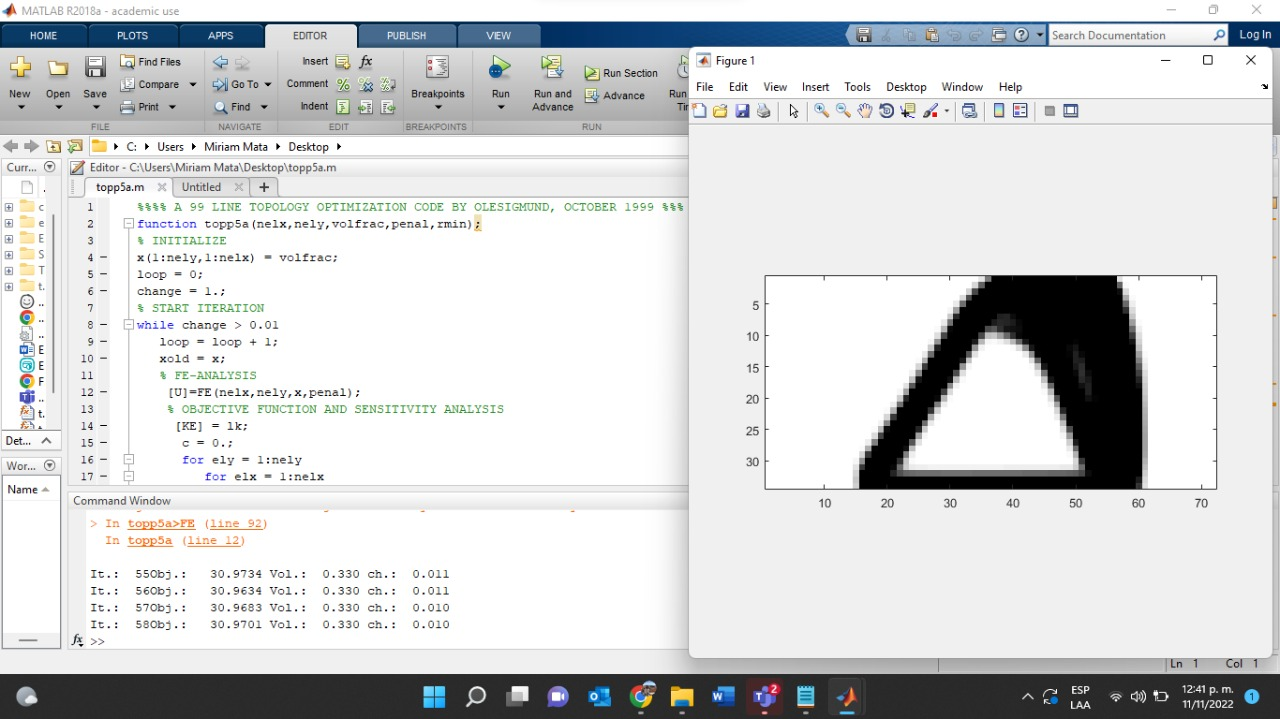
\includegraphics[width=150mm]{oar.jpeg} % archivo
    \caption{Vista completa del resultado del código A.}
    \label{grafica}
\end{figure}
\begin{figure}[htp]
  \centering
  \subfloat[]{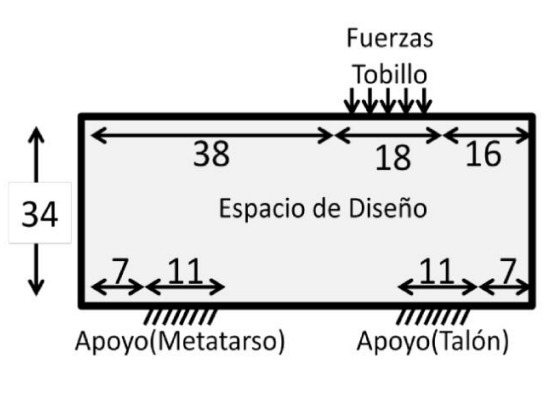
\includegraphics[width=0.4\textwidth]{f1 Normal.jpeg}\label{fig:f1}}
  \hfill
  \subfloat[]{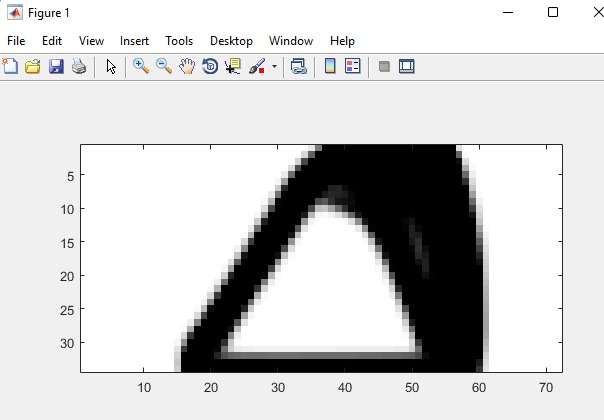
\includegraphics[width=0.4\textwidth]{ra.jpeg}\label{fig:f2}}
  \caption{F1 posición normal y su resultado.}
\end{figure}
\newpage
\begin{figure}[htp] % figura
    \centering
    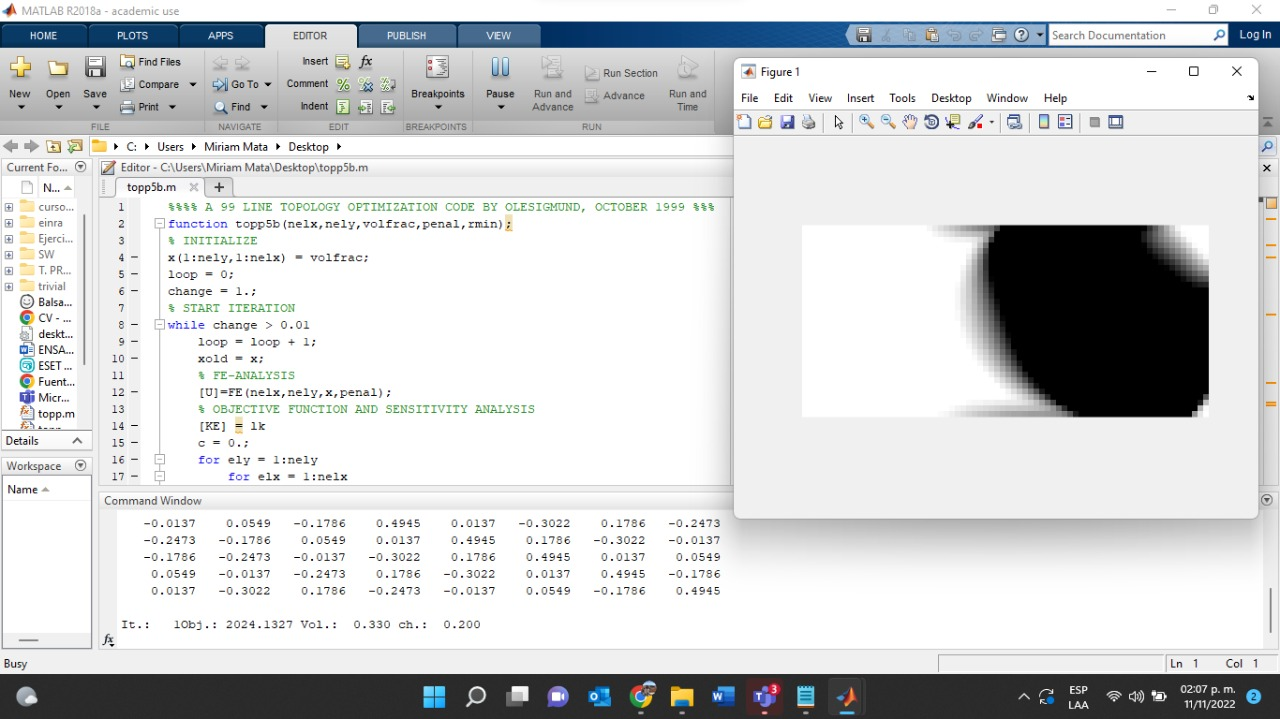
\includegraphics[width=150mm]{obr.jpeg} % archivo
    \caption{Vista completa del resultado del código B.}
    \label{grafica}
\end{figure}
\begin{figure}[htp]
  \centering
  \subfloat[]{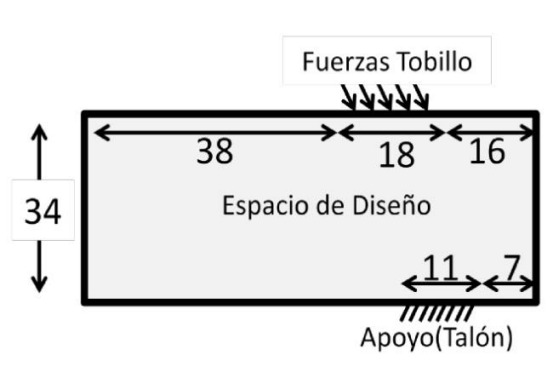
\includegraphics[width=0.4\textwidth]{f2 Despegue.jpeg}\label{fig:f1}}
  \hfill
  \subfloat[]{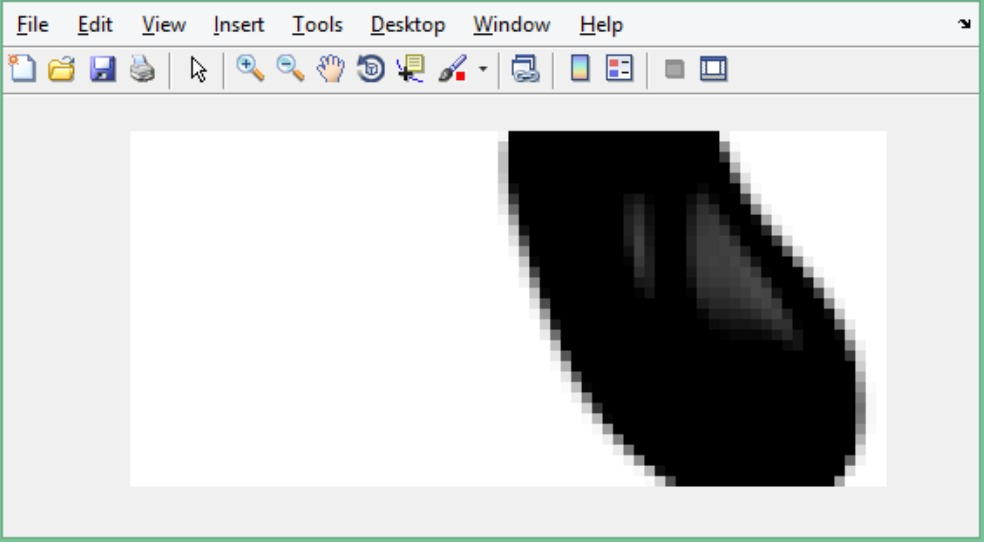
\includegraphics[width=0.4\textwidth]{rb.jpeg}\label{fig:f2}}
  \caption{F2 posición de despegue y su resultado.}
\end{figure}
\newpage
\begin{figure}[htp] % figura
    \centering
    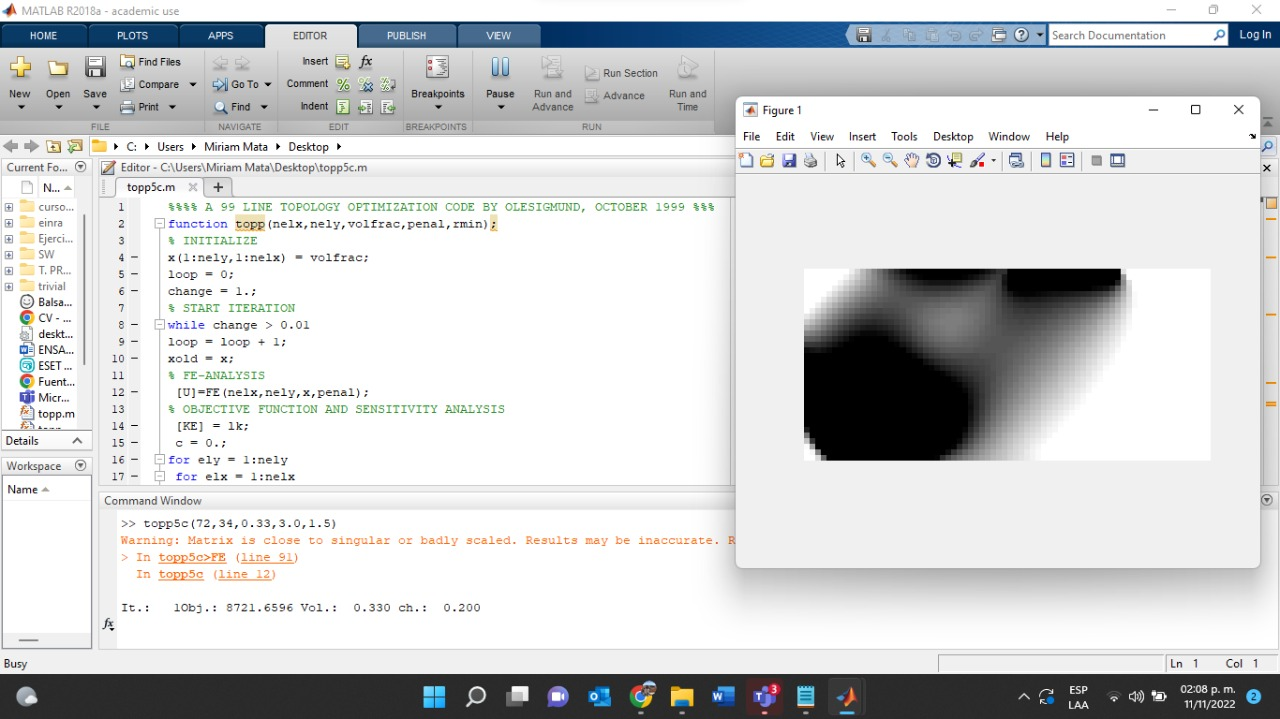
\includegraphics[width=150mm]{ocr.jpeg} % archivo
    \caption{Vista completa del resultado del código C.}
    \label{grafica}
\end{figure}
\begin{figure}[htp]
  \centering
  \subfloat[]{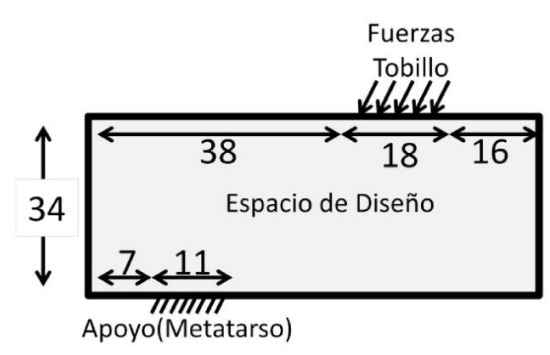
\includegraphics[width=0.4\textwidth]{f3 Apoyo.jpeg}\label{fig:f1}}
  \hfill
  \subfloat[]{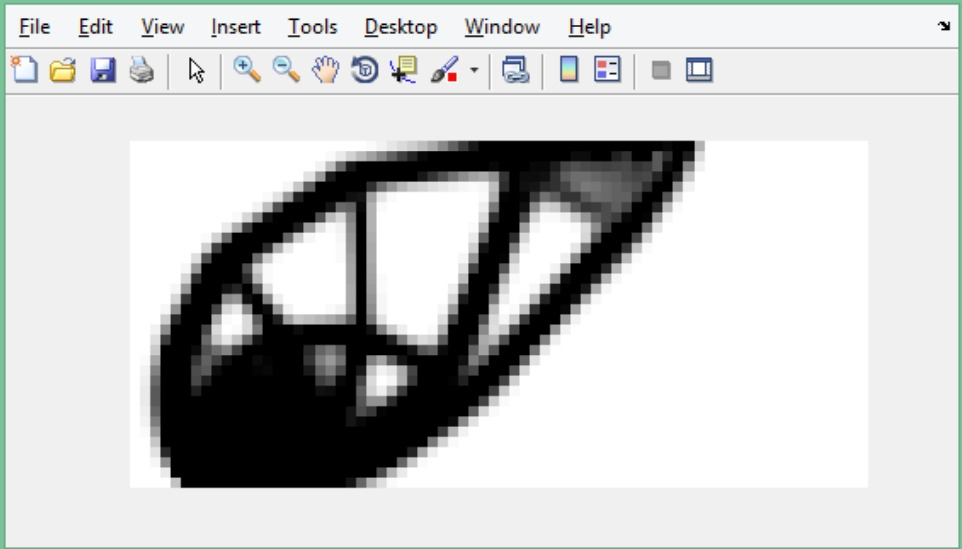
\includegraphics[width=0.4\textwidth]{rc.jpeg}\label{fig:f2}}
  \caption{F2 posición de apoyo y su resultado.}
\end{figure}
 \newpage
\section{Conclusiones}
\subsection{Jorge  Fuentes}
En esta ocasión tratando de cumplir el objetivo planteado de presentar una propuesta de análisis de formas y de la programación para la ejecución de la optimización de características de trabajo especificas que presenta las ventajas ahora en esta práctica 5 sobre la elaboración de una Optimización de una prótesis de pie, aplicando los conocimientos previos sobre nuestro dominio en MATLAB así como los pasos de la programación logramos elaborar una Optimización resultante para una prótesis de pie.
\subsection{Tania  Hernandez}
La práctica realizada consistió en la elaboración de una prótesis de pie, para la cual como en todas las anteriores prácticas, es por esto, que se tuvo que investigar la forma geométrica,  estado del arte,entre otros aspectos relevantes, de mi parte aprendí, que se pueden realizar distintos tipos de formas de diseño del pie, el cual varia dependiendo las necesidades aue ocupe el paciente y la optatizacion en MATLAB..
\subsection{Anahi Herrera}
Para esta actividad se realizaron varias búsquedas de información para ver las características de este trabajo final, por lo cual, se recopilaron los conocimientos adquiridos durante todo el curso y gracias a ellos fue que se logró con este último objetivo de realizar el diseño de una prótesis de pie.\\ 
De igual manera para llegar al resultado se tuvieron que realizar investigaciones sobre el funcionamiento de este tipo de prótesis, algunos modelos comerciales ya realizados para así obtener resultados positivos en nuestro trabajo. 

\subsection{Gustavo  Díaz}
Dentro de la investigación requerida para el desarrollo de la practica fue un poco sencillo de encontrar la información dado que dentro de la clase se nos pedía encontrar información de esta rama de la biomecánica dado que las prótesis son una forma en que se aplica a la perfección esta rama de la mecánica, en la cual para poder mejorar dicha prótesis se uso el software de Matlab en el cual se buscaron las diferente partes en las cuales se puede optimizar de manera correcta y que no afecte la estructura de la misma, y sea sencilla para el fabricante hacerla y sea sencilla y cómoda de usar. 
\subsection{Miriam  Mata}
Durante este curso de laboratorio mi equipo y yo nos dimos cuenta que se puede usar Matlab para generar un análisis de elemento finito para objetos de ámbito simple y que se pueden usar para diferentes casos, además de generar un buen soporte que nos ayudará mucho en este caso. A partir de lo que aprendimos, nos damos cuenta que los softwares de hoy en día nos apoyan mucho con cálculos e impresiones que nos facilitan el poder generar nuevas ideas e ir más rápido en nuestras investigaciones.
\subsection{Alejandro Ramos}
En esta práctica pude observar para empezar el diseño de una prótesis de pie despues observamos como la podríamos mejorar
de diferentes maneras hasta que decidimos una, lo cual fue complicado porque para eso tuvimos que investigar bastante 
porque no es tan sencillo mejorarlas debido a que un error y podemos causar daño a la persona que la usara
pero para mi si la mejoramos de la manera correcta y espero seguir aprendiendo proque me interesa bastante
esta área de biomecánica.
\bibliography{bib}
\bibliographystyle{plainnat}
\end{document}
